\documentclass{article}

% Título del artículo
\title{Números reales}
\author{Edwin Leonel Lee Tiño}
\date{\today}

% Paquetes configurar página
\usepackage[margin=2.5cm]{geometry}
\usepackage{parskip}
\usepackage{xcolor}
\usepackage{float}

% Paquetes matemáticos
\usepackage{amsmath}
\usepackage{amssymb}
\usepackage{amsthm}

% Paquetes para gráficos
\usepackage{pgfplots}
\pgfplotsset{compat=1.18}
\usepgfplotslibrary{fillbetween}
\usepackage{tikz}
\usetikzlibrary{patterns}

% Nota
\usepackage[framemethod=default]{mdframed}
\newenvironment{nota_computacional}
  {\begin{mdframed}[backgroundcolor=gray!10, linecolor=gray!40, roundcorner=5pt, skipabove=10pt, skipbelow=10pt]}
  {\end{mdframed}}

% --- Inicio del documento ---
\begin{document}
\maketitle

\section{Axiomas de campo}

Los números reales, junto con las operaciones de \textbf{suma} ($+$) y \textbf{multiplicación} ($\times$), satisfacen una serie de propiedades conocidas como \textbf{axiomas de campo}. Estas son la definición formal de por qué el álgebra funciona.

\subsection{Axiomas de adición}

\begin{itemize}
    \item \textbf{Clausura:} Si $a, b \in \mathbb{R}$, entonces $a + b \in \mathbb{R}$.
    \item \textbf{Asociativa:} Sean $a, b, c \in \mathbb{R}$, se tiene que $(a + b) + c = a + (b + c)$.
    \item \textbf{Conmutativa:} Sean $a, b \in \mathbb{R}$ se cumple que $a + b = b + a$.
    \item \textbf{Elemento neutro:} Existe un elemento $0 \in \mathbb{R}$, tal que $a + 0 = a, \ \forall a \in \mathbb{R}$.
    \item \textbf{Elemento inverso:} Para cada $a \in \mathbb{R}$, existe un elemento $-a \in \mathbb{R}$, tal que $a + (-a) = 0$. 
\end{itemize}

\subsection{Axiomas de multiplicación}

\begin{itemize}
    \item \textbf{Clausura:} Si $a, b \in \mathbb{R}$, entonces $a \times b \in \mathbb{R}$.
    \item \textbf{Asociativa:} Sean $a, b, c \in \mathbb{R}$, se tiene que $(a \times b) \times c = a \times (b \times c)$.
    \item \textbf{Conmutativa:} Sean $a, b \in \mathbb{R}$ se cumple que $a \times b = b \times a$.
    \item \textbf{Elemento neutro:} Existe un elemento $1 \in \mathbb{R}$, tal que $a \times 1 = a, \ \forall a \in \mathbb{R}$.
    \item \textbf{Elemento inverso:} Para cada $a \in \mathbb{R}$, con $a \neq 0$, existe un elemento $a^{-1} \in \mathbb{R}$, tal que $a \times a^{-1} = 1$. 
\end{itemize}

\textbf{Axioma distributivo:} Sean $a, b, c \in \mathbb{R}$, se tiene que $a \times (b + c) = (a \times b) + (a \times c)$.

\textit{Ejemplo:}

Demostrar que si $a + b = a$, entonces $b = 0$

Sumar \textbf{inverso aditivo} en ambos lados de la ecuación:

$(a + b) + (-a) = a + (-a)$

Por \textbf{asociatividad} y \textbf{conmutatividad} se tiene que:

$(a + (-a)) + b = a + (-a)$


Por axioma de \textbf{inverso aditivo} se tiene:

$0 + b = 0$

Finalmente, por axioma de \textbf{neutro aditivo} se obtiene que:

$b = 0$ $\qed$

\textit{Ejemplo:}

Demostrar que el \textbf{neutro aditivo} es único.

Suponer que existe otro neutro aditivo $0' \in \mathbb{R}$, tal que $0 \neq 0'$.

Por axioma de \textbf{neutro aditivo} se tiene:

$0 + 0' = 0$

Pero como $0$ también es neutro aditivo, aplica nuevamente el axioma de \textbf{neutro aditivo}:

$0' + 0 = 0'$

Por axioma \textbf{conmutativo} se sabe:

$0 + 0' = 0' + 0 \implies 0 = 0'$

Se ha llegado a una \textbf{contradicción}, por lo tanto, la proposición sobre que existe otro neutro aditivo es falso.

$\qed$

\textit{Ejemplo:}

Demostrar que el \textbf{neutro multiplicativo} es único.

Suponer que existe otro neutro multiplicativo $1' \in \mathbb{R}$, tal que $1' \neq 1$.

Por axioma de \textbf{neutro multiplicativo} se tiene que:

$1 \times 1' = 1$

Pero como $1$ también es neutro multiplicativo, se aplica el axioma de \textbf{neutro multiplicativo}:

$1' \times 1 = 1'$

Por axioma \textbf{conmutativo} se tiene:

$1 \times 1' = 1' \times 1 \implies 1 = 1'$

Esto es una \textbf{contradicción}, entonces, la proposición inicial sobre que existe otro neutro multiplicativo no es verdadero.

$\qed$

\section{Axiomas de orden}

\begin{itemize}
    \item \textbf{Tricotomía:} Para cualquiera $a, b \in \mathbb{R}$, solo una de las siguientes proposiciones es verdadera: 
    
    $a < b$, $a > b$ o $a = b$.
    \item \textbf{Transitividad:} Sean $a, b, c \in \mathbb{R}$, si $a < b$ y $b < c$, entonces $a < c$.
    \item \textbf{Compatibilidad con la adición:} Sean $a, b, c \in \mathbb{R}$, si $a < b$, entonces $a + c < b + c$, para cualquier $c$.
    \item \textbf{Compatibilidad con el producto:} Para $a, b, c \in \mathbb{R}$, si $a < b$ y $c > 0$ se tiene que $a \times c < b \times c$.
\end{itemize}

A partir de estos axiomas, se definen los \textbf{intervalos}, que serán fundamentales en Cálculo para definir dominios y rangos:

\begin{itemize}
    \item \textbf{Abierto:} $(a, b) = \{x \mid a < x < b\}$
    \item \textbf{Cerrado:} $[a, b] = \{x \mid a \le x \le b\}$
    \item \textbf{Semiabiertos:} $(a, b] = \{x \mid a < x \le b\}$
    \item \textbf{Infinitos:} $(a, \infty)$ y $(-\infty, b)$
\end{itemize}

\section{Valor absoluto y recta real}

El valor absoluto es una \textbf{función} que mide la distancia.

\textbf{Definición formal:}

\[ 
\mid x \mid =  
\begin{cases}
    x \text{ si } x \ge 0 \\
    -x \text{ si } x < 0    
\end{cases}
\]

\textbf{Interpretación geométrica:}

$\mid x \mid$ es la distancia entre el punto $x$ y el origen $0$ en la recta real.

\begin{figure}[ht]
    \centering
    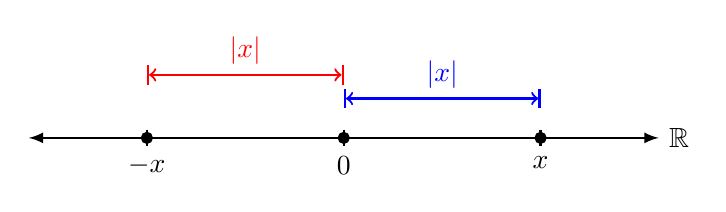
\begin{tikzpicture}[extended line/.style={shorten >=-#1,shorten <=-#1},
                        extended line/.default=1cm]
        % Dibujo de la recta numérica
        \draw[latex-latex, thick] (-4,0) -- (4,0) node[right] {$\mathbb{R}$};
        % Marcas principales: 0 y x
        \draw[shift={(0,0)}, thick] (0pt,3pt) -- (0pt,-3pt) node[below] {$0$};
        \draw[shift={(2.5,0)}, thick] (0pt,3pt) -- (0pt,-3pt) node[below] {$x$};
        \draw[shift={(-2.5,0)}, thick] (0pt,3pt) -- (0pt,-3pt) node[below] {$-x$};
        % Representación de la distancia |x| (derecha)
        \draw[|<->|, blue, thick] (0,0.5) -- (2.5,0.5) node[midway, above] {$|x|$};
        % Representación de la distancia |x| (izquierda) para mayor claridad
        \draw[|<->|, red, thick] (0,0.8) -- (-2.5,0.8) node[midway, above] {$|x|$};
        % Puntos destacados
        \filldraw[black] (0,0) circle (2pt);
        \filldraw[black] (2.5,0) circle (2pt);
        \filldraw[black] (-2.5,0) circle (2pt);
    \end{tikzpicture}
    \caption{Interpretación geométrica del valor absoluto como distancia al origen.}
\end{figure}

Más generalmente, $\mid x - a \mid$ es la distancia entre $x$ y $a$.

\textbf{Propiedades:}

\begin{enumerate}
    \item $\mid x \mid \ge 0$, para todo $x \in \mathbb{R}$ y $\mid x \mid = 0 \iff x = 0$.
    \item $\mid x \times y \mid = \mid x \mid \times \mid y \mid$.
    \item \textbf{Desigualdad triangular:} $\mid x + y \mid \le \mid x \mid + \mid y \mid$.
    \item $\mid x \mid < a \iff -a < x < a$.
    \item $\mid x \mid > a \iff x > a \lor x < -a$.
\end{enumerate}

\textit{Ejemplo:}

Demostrar que $\mid x + y \mid \le \mid x \mid + \mid y \mid$

\underline{Caso No. 1:}

Se supondrá que $x, y \ge 0$

Por definición de \textbf{valor absoluto} se sabe:

$\mid x + y \mid = x + y$

$\mid x \mid = x \ \land \  \mid y \mid = y \implies \mid x \mid + \mid y \mid = x + y$

Implica que: 

$\mid x + y \mid = \mid x \mid + \mid y \mid$

\underline{Caso No. 2:}

Suponer que $x, y < 0$

Nuevamente, por definición de \textbf{valor absoluto} se tiene que:

$\mid x + y \mid = - (x + y) = - x - y$

$\mid x \mid = - x \ \land \ \mid y \mid = - y \implies \mid x \mid + \mid y \mid = - x - y$

Por lo tanto: 

$\mid x + y \mid = \mid x \mid + \mid y \mid$

\underline{Caso No. 3:}

Se supone que $x \ge 0$ y $y < 0$ (o viceversa).

Se pueden dar dos escenarios posibles:

a) Si $x + y > 0$

Por definición de \textbf{valor absoluto} se tiene:

$\mid x + y \mid = x + y$

$\mid x \mid = x \ \land \ \mid y \mid = - y \implies \mid x \mid + \mid y \mid = x + (- y)$

Como $y < 0 \implies -y > 0 \implies y < - y$

Sumar $x$ en ambos lados de la desigualdad:

$x + y < x + (- y) \implies \mid x + y \mid < \mid x \mid + \mid y \mid$

b) Si $x + y < 0$

Otra vez, por definición de \textbf{valor absoluto} se obtienen los siguientes resultados:

$\mid x + y \mid = -(x + y) = - x - y$

Ya se sabe que $\mid x \mid + \mid y \mid = x + (- y)$

Como $x \ge 0 \implies -x \le 0 \implies -x \le x$

Sumar $- y$ en ambos lados de la desigualdad:

$- x - y \le x + (-y)$

La única manera que se de $- x - y = x + (- y)$, es que $y = 0$, pero se sabe que $y < 0$, por lo tanto:

$- x - y < x + (-y)$

$\qed$

\textit{Ejemplo:}

Generar la demostración para $\mid x \mid < a \iff - a < x < a$

$(\implies)$ PD: $\mid x \mid \ < a \implies -a < x < a$

Se pueden dar dos posibles casos:

a) Si $x \ge 0 \implies \mid x \mid = x$

Entonces:

$\mid x \mid < a \implies x < a$

Como $x \ge 0 \ \land \ x < a \implies a > 0 \implies -a < 0$

Por lo tanto:

$\mid x \mid < a \implies - a < x < a$

b) Si $x < 0 \implies \mid x \mid = - x$

Se tiene que:

$\mid x \mid < a \implies - x < a$

Como $x < 0 \implies - x > 0$, además se sabe que $- x < a \implies a > 0 \implies x < a$.

Sumar $x$ a la desigualdad $- x < a$:

$- x + x < a + x $

Por axioma de \textbf{inverso aditivo} se obtiene:

$0 < a + x$

Sumar $- a$ a la nueva desigualdad:

$0 + (-a) < (a + x) + (-a)$

Por axiomas \textbf{conmutativo} y \textbf{asociativo} se obtiene:

$0 + (-a) < (a + -(a)) + x$

Por axiomas de \textbf{inverso y neutro aditivo} se logra:

$-a < x$

Por lo tanto:

$\mid x \mid < a \implies -a < x < a$

$(\impliedby)$ PD: $-a <  x  < a \implies \mid x \mid < a$

Se consideran dos escenarios:

a) Si $x \ge 0 \implies \mid x \mid = x$

Como $x \ge 0 \ \land \ x < a \implies a > 0 \implies - a < 0$

Se cumple $-a < x < a \implies \mid x \mid < a$

b) Si $x < 0 \implies \mid x \mid = - x > 0$

Se sabe que $-a < x$, sumar $a$ a la desigualdad:

$- a + a < x + a$

Por axioma de \textbf{inverso aditivo} se tiene:

$0 < x + a$, luego sumar $-x$ a la desigualdad:

$0 + (-x) < (x + a) + (-x)$

Por axiomas \textbf{asociativo} y \textbf{conmutativo} se puede operar:

$0 + (-x) < (x + (-x)) + a$

Por axiomas de \textbf{inverso y neutro aditivo} se obtiene:

$- x < a \implies \mid x \mid < a$

$\qed$

\textit{Ejemplo:}

Demostrar que $\mid x \mid > a \iff x > a \ \lor \ x < - a$

$(\implies)$ PD: Si $\mid x \mid > a \implies x > a \ \lor \ x < -a$

\underline{Caso No. 1:}

Si $x \ge 0 \implies \mid x \mid = x$

Entonces, se tiene $\mid x \mid > a \implies x > a$

\underline{Caso No. 2:}

Si $x < 0 \implies \mid x \mid = - x$

Se tiene que $\mid x \mid > a \implies -x > a$

Sumar $x$ en la desigualdad:

$- x + x > a + x$

Por axioma de \textbf{inverso aditivo} se tiene:

$0 > x + a$

Se suma $- a$ en la nueva desigualdad:

$0 + (-a) > (x + a) + (-a)$

Se aplica axiomas \textbf{conmutativo} y \textbf{asociativo}:

$0 + (-a) > (a + (-a)) + x$

Por axioma de \textbf{inverso aditivo} se obtiene:

$-a > x \implies x < -a$

$(\impliedby)$ PD: si $x > a \ \lor \ x < - a \implies \mid x \mid > a$

\underline{Caso No. 1:}

Si $x \ge 0 \implies \mid x \mid = x$

Como $x > a \implies \mid x \mid > a$

\underline{Caso No. 2:}

Si $x < 0 \implies \mid x \mid = -x$

Como $x < - a$, sumar $- x$ a la desigualdad:

$x + (-x) < - a + (-x)$

Aplicar axioma de \text{inverso aditivo}:

$0 < -a + (-x)$

Sumar $a$ a la nueva desigualdad:

$0 + a < (-a + (-x)) + a$

Por axiomas \textbf{asociativo} y  \textbf{conmutativo} se tiene:

$0 + a < (-a + a) + (-x)$

Se aplican los axiomas de \textbf{inverso y neutro aditivo}:

$a < - x \implies -x > a \implies \mid x \mid > a$

$\qed$

\section{Desigualdades con valor absoluto}

El valor absoluto no permite resolver dos tipos fundamentales de desigualdades, que aparecen al calcular límites, especialmente los \textbf{límites epsilon-delta}:

\begin{itemize}
    \item Desigualdad de la forma $\mid x - a \mid < c$
    \begin{itemize}
        \item Significado geométrico: La distancia entre $x$ y $a$ es menor que $c$.
        \item Solución: Se tiene que $\mid x - a \mid < c \implies -c < x - a < c$.
    \end{itemize}
    \item Desigualdad de la forma $\mid x - a \mid > c$
    \begin{itemize}
        \item Significado geométrico: La distancia entre $x$ y $a$ es mayor que $c$.
        \item Solución: Se tiene $\mid x - a \mid > c \implies (x - a) > c \ \lor \ (x - a) < - c$.
    \end{itemize}
\end{itemize}

\section{Problemas aplicados}

\textbf{1. Análisis de errores en punto flotante:} En computación, los números reales se aproximan usando un sistema de punto flotante debido a las limitaciones físicas de la memoria. Si $x$ es el valor real exacto y $\hat{x}$ es el valor aproximado almacenado en memoria, el \textbf{error relativo} está acotado superiormente por una máquina epsilon $(\epsilon > 0)$ mediante la siguiente desigualdad:

$\displaystyle \left| \frac{x - \hat{x}}{x} \right| < \epsilon \text{ con } x \neq 0$

Utilizando las propiedades de valor absoluto y los axiomas de orden, demostrar que el valor aproximado $\hat{x}$ se encuentra obligatoriamente confinado dentro del intervalo abierto:

$\Big(x(1 - \epsilon), x(1 + \epsilon)\Big) \text{ para el caso que } x > 0$

Dada la desigualdad $\displaystyle \left| \frac{x - \hat{x}}{x} \right| < \epsilon$, por propiedad (4) de \textbf{valor absoluto} se tiene:

$\displaystyle \left| \frac{x - \hat{x}}{x} \right| < \epsilon \implies -\epsilon < \frac{x - \hat{x}}{x} < \epsilon$

Multiplicar la desigualdad por $x$:

$\displaystyle -\epsilon(x) < \frac{x - \hat{x}}{x} \times x < \epsilon(x) \implies -\epsilon(x) < x - \hat{x} < \epsilon(x)$

Sumar $- x $ a la nueva desigualdad:

$-\epsilon(x) + (- x) < (x - \hat{x}) + (- x) < \epsilon(x) + (-x)$

Se aplican axiomas \textbf{asociativo} y \textbf{conmutativo}:

$(- x) -\epsilon(x) < (x + (- x)) - \hat{x} < (-x) + \epsilon(x)$

Mediante axioma de \textbf{inverso aditivo} se obtiene:

$(- x) -\epsilon(x) < - \hat{x} < (-x) + \epsilon(x)$

Multiplicar $-1$ a la desigualdad actual:

$-1 ((- x) -\epsilon(x)) < -1 (- \hat{x}) < -1 ((-x) + \epsilon(x))$

Recordar que al multiplicar por un número negativo, cambia el sentido de la desigualdad:

$x + \epsilon(x) > \hat{x} > x - \epsilon(x) \implies x - \epsilon(x) < \hat{x} < x + \epsilon(x)$

Se aplica \textbf{factor común}:

$x(1 - \epsilon) < \hat{x} < x(1 + \epsilon)$

$\qed$

\textbf{2. Complejidad algorítmica y cotas de rendimiento:} El tiempo de ejecución de un algoritmo de ordenamiento en el peor de los casos está modelado por una función $T(n)$, donde $n$ representa la cantidad de datos a procesar. Se ha determinado experimentalmente que el rendimiento real de este algoritmo satisface la condición:

$\mid T(n) - c \times n^2 \mid \le k \times n$

Donde $c$ y $k$ son constantes positivas que dependen de la arquitectura del procesador. Utilizar la \textbf{desigualdad triangular} para demostrar que el tiempo total de ejecución $T(n)$ está acotado superiormente por la función cuadrática:

$T(n) \le c \times n^2 + k \times n$

Se tiene la siguiente identidad:

$T(n)  = (T(n) - c \times n^2) + c \times n^2$

Se aplica \textbf{valor absoluto} en ambos lados de la igualdad:

$\mid T(n) \mid  = \mid (T(n) - c \times n^2) + c \times n^2 \mid$

Por \textbf{desigualdad triangular} se obtiene:

$\mid (T(n) - c \times n^2) + c \times n^2 \mid \le \mid T(n) - c \times n^2 \mid + \mid c \times n^2 \mid$

Entonces:

$\mid T(n) \mid \le \mid T(n) - c \times n^2 \mid + \mid c \times n^2 \mid$

Restar $\mid c \times n^2 \mid$ en la desigualdad actual:

$\mid T(n) \mid - \mid c \times n^2 \mid \le \mid T(n) - c \times n^2 \mid + \mid c \times n^2 \mid - \mid c \times n^2 \mid \implies \mid T(n) \mid - \mid c \times n^2 \mid  \le \mid T(n) - c \times n^2 \mid$

Como $\mid T(n) - c \times n^2 \mid \le k \times n$, por axioma de \textbf{transitividad} se tiene que:

$\mid T(n) \mid - \mid c \times n^2 \mid \le k \times n$

Es sabido que $c \times n^2 > 0$, además se supone que el tiempo de ejecución de un algoritmo es mayor que cero, por lo tanto, se tiene que:

$T(n) - c \times n^2 \le k \times n \implies T(n) \le c \times n^2 + k \times n$

$\qed$

\textbf{3. Criterio de parada en algoritmos numéricos (convergencia):} Un script de programación implementa un método numérico iterativo para aproximar la raíz de una función. El criterio de parada dentro del bucle de control (while) exige que la aproximación actual $x_k$ y la aproximación del paso anterior $x_{k - 1}$ cumplan la condición de cercanía:

$\mid x_k - x_{k - 1} \mid < \delta$

Donde $\delta$ es la tolerancia de precisión del programa. Si en una iteración específica el algoritmo registra $x_{k - 1} = L$, demostrar analíticamente (usando las propiedades de intervalos abiertos para el valor absoluto) qué rango estricto de valores permitidos puede tomar $x_k$ para que el programa rompa el ciclo y finalice su ejecución con éxito. 

\begin{nota_computacional}
\underline{Nota:}

La \textbf{raíz} de una función $f(x)$ es el valor de $x$ que hace que la función sea igual que cero. Matemáticamente:

$f(x) = 0$

El \textbf{método Newton-Raphson} es un algoritmo diseñado para encontrar raíces de funciones de forma numérica cuando no es fácil despejar la $x$. El algoritmo funciona de la siguiente manera:

\begin{enumerate}
    \item Se hace una estimación inicial $x_{k - 1}$.
    \item El algoritmo calcula una nueva aproximación $x_k$, que debería estar más cerca de la raíz. Se usa la ecuación:
    
    $\displaystyle x_k = x_{k - 1} - \frac{f(x_{k - 1})}{f'(x_{k - 1})}$.

    \item Se repite el proceso hasta que la diferencia sea menor a un nivel de tolerancia dado $\delta$:
    
    $\mid x_k - x_{k - 1} \mid < \delta$

\end{enumerate}

Por ejemplo, suponer la función $f(x) = x^2 - 2$, de la cual se sabe su raíz es $\sqrt{2} \approx 1.41421$.

Además, la derivada de la función $f(x)$ es $f'(x) = 2x$.

Se puede pensar en una primera estimación $x_{k - 1} = 1$.

Se encuentra una nueva estimación (que debe estar más cerca a $\sqrt{2}$), mediante la ecuación:

$\displaystyle x_k = 1 - \frac{(1)^2 - 2}{2(1)} = 1 + 0.5 = 1.5$.

Calcular la diferencia entre estimaciones y compararla con un nivel de tolerancia $\delta = 0.01$:

$\mid 1.5 - 1 \mid < 0.01 \implies 0.5 < 0.01$

Como no se cumple, se procede a calcular una nueva estimación:

$\displaystyle x_k = 1.5 - \frac{(1.5)^2 - 2}{2(1.5)} = 1.5 - \frac{1}{12} = \frac{17}{12} \approx 1.417$.

Nuevamente, se compara la diferencia de estimaciones con $\delta$:

$\mid \frac{17}{12} - 1.5 \mid < 0.01 \implies \frac{1}{12} \approx 0.083 < 0.01$

De nuevo no cumple con la desigualdad, entonces, se vuelve a encontrar un nuevo estimador:

$\displaystyle x_k = \frac{17}{12} - \frac{(\frac{17}{12})^2 - 2}{2(\frac{17}{12})} = \frac{17}{12} - \frac{1}{408} = \frac{577}{408} \approx 1.41422$

Se compara la diferencia de estimaciones versus el nivel de tolerancia:

$\mid \frac{577}{408} - \frac{17}{12}\mid < 0.01 \implies \frac{1}{408} \approx 0.0025 < 0.01$

Se cumple la desigualdad, por lo tanto, se rompe la \textbf{iteración} y se puede concluir que la raíz de la función $f(x)$ aproximadamente $1.41422$, con un nivel de tolerancia del $1\%$.

\end{nota_computacional}

Dado $x_{k - 1} = L$ se tiene:

$\mid x_k - L \mid < \delta$

Por propiedad (4) de \textbf{valor absoluto} se tiene que:

$\mid x_k - L \mid < \delta \implies -\delta < x_k - L <  \delta$

Sumar $L$ en la desigualdad actual:

$-\delta + L < (x_k - L) + L <  \delta + L$

Por axioma de \textbf{inverso aditivo} y \textbf{conmutatividad} se obtiene:

$L -\delta < x_k < L + \delta$

Por lo tanto, para que la diferencia entre las estimaciones "rompa" con el bucle, dado un nivel de tolerancia $\delta$, debe estar en el rango $(L -\delta, L + \delta)$.

$\qed$

\textbf{4. Distancia de Hamming y transmisión de datos:} En la teoría de redes y comunicación de datos, la fidelidad de una señal suele modelarse  mediante distancias. Si se analiza un flujo unidimensional de bits donde $x$ representa la intensidad de la señal analógica recibida y $a$ es el umbral de sincronización ideal, un \textbf{bit erróneo (ruido)} se registra en el sistema cuando la señal se desvía demasiado:

$\mid x - a \mid < \gamma$

Donde $\gamma$ es la tolerancia máxima de ruido del canal físico. Descomponer formalmente esta condición en sus dos intervalos disjuntos de falla de datos, aplicando la propiedad de colas infinitas del valor absoluto.

El escenario de falla de datos está dado por: $\mid x - a \mid > \gamma$.

En otras palabras, cuando la diferencia entre la intensidad y el umbral es mayor que la tolerancia máxima $\gamma$.

Por propiedad (5) de \textbf{valor absoluto} se tiene que:

$\mid x - a \mid > \gamma \implies x - a > \gamma \ \lor \ x - a < -\gamma$

Sumar $a$ en ambas desigualdades:

$(x - a) + a > \gamma + a \ \lor \ (x - a) + a < - \gamma + a$

Por propiedad \textbf{conmutativa} y \textbf{asociativa} se obtiene:

$(a - a) + x > a + \gamma \ \lor \ (a - a) + x < a - \gamma$

Por axioma de \textbf{inverso aditivo}:

$x > a + \gamma \ \lor \ x < a - \gamma \implies (-\infty, a - \gamma) \cup (a + \gamma, +\infty)$

$\qed$

\textbf{5. Estabilidad en gráficos por computadora (Bounding boxes):} Un motor renderizado de videojuegos 2D evalúa si un personaje se encuentra dentro del rango de iluminación difusa de una antorcha situada exactamente en el origen 0. La condición matemática para que reciba luz en el eje horizontal exige que $\mid x \mid < R$, donde $R$ es el radio de alcance de la luz.

Si una ráfaga de viento en el juego altera repentinamente la posición del personaje sumándole un factor de perturbación $\Delta x$, demostrar empleando la \textbf{desigualdad triangular} que el nuevo estado del personaje estará plenamente iluminado si el motor gráfico garantiza de antemano la siguiente condición:

$\mid x \mid + \mid \Delta x \mid < R$

\begin{figure}[H]
\centering
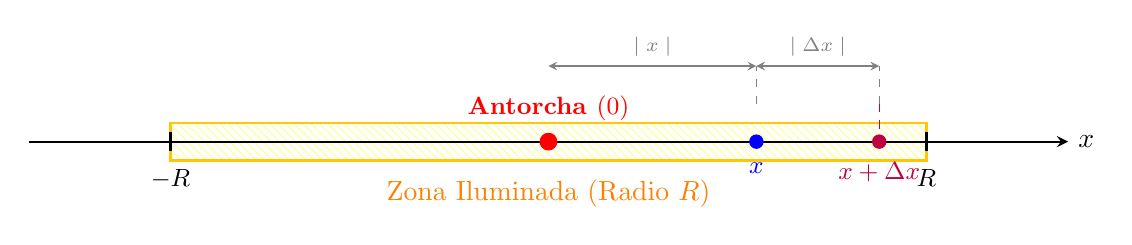
\begin{tikzpicture}[scale=1.2]
    % Definición de estilos
    \tikzstyle{axis}=[>=stealth, ->, thick, black]
    \tikzstyle{lightzone}=[pattern=north west lines, pattern color=yellow!40, draw=yellow!60!orange, thick]
    % Dibujo de la zona de iluminación (Radio R desde el origen)
    % Representa el intervalo abierto (-R, R)
    \fill[lightzone] (-4, -0.2) rectangle (4, 0.2);
    \node[orange, below] at (0, -0.3) {Zona Iluminada (Radio $R$)};
    % Eje horizontal (Eje X del mapa)
    \draw[axis] (-5.5,0) -- (5.5,0) node[right] {$x$};
    % Marcas del Radio R en el eje
    \draw[thick] (4,0.1) -- (4,-0.1) node[below=3pt, font=\small] {$R$};
    \draw[thick] (-4,0.1) -- (-4,-0.1) node[below=3pt, font=\small] {$-R$};
    % El Origen (Posición de la Antorcha)
    \filldraw[red] (0,0) circle (2.5pt);
    \node[red, above=4pt, font=\small\bfseries] at (0,0) {Antorcha $(0)$};
    % Posición original del personaje (x)
    \coordinate (X) at (2.2, 0);
    \filldraw[blue] (X) circle (2pt);
    \node[blue, below=4pt, font=\small] at (X) {$x$};
    % Nueva posición real del personaje (x + \Delta x)
    \coordinate (Xnew) at (3.5, 0);
    \filldraw[purple] (Xnew) circle (2pt);
    \node[purple, below=4pt, font=\small\bfseries] at (Xnew) {$x + \Delta x$};
    % Línea punteada que conecta la posición alterada al eje
    \draw[dashed, purple] (3.5, 0.4) -- (3.5, 0);
    % Cota de distancia de la Desigualdad Triangular
    % Indica visualmente que |x| + |\Delta x| < R mantiene todo dentro de la zona sombreada
    \draw[<->, >=stealth, gray, thin] (0, 0.8) -- (2.2, 0.8) node[midway, above, font=\scriptsize] {$\mid x \mid$};
    \draw[<->, >=stealth, gray, thin] (2.2, 0.8) -- (3.5, 0.8) node[midway, above, font=\scriptsize] {$\mid \Delta x \mid$};
    \draw[dashed, gray] (2.2, 0.4) -- (2.2, 0.8);
    \draw[dashed, gray] (3.5, 0.4) -- (3.5, 0.8);
\end{tikzpicture}
\caption{Iluminación de personaje considerando factor de perturbación (viento).}
\label{fig:bounding_box}
\end{figure}

La nueva distancia del personaje en relación al origen (antorcha) estaría dado por:

$\mid x + \Delta x \mid$

Por propiedad \textbf{desigualdad triangular} es sabido que:

$\mid x + \Delta x \mid \le \mid x \mid + \mid \Delta x \mid$

Como el motor gráfico garantiza que $\mid x \mid + \mid \Delta x \mid < R$, por \textbf{transitividad} se obtiene:

$\mid x + \Delta x \mid < R$

$\qed$

\end{document} 